\documentclass[12pt,a4paper]{article}
\usepackage[a4paper]{geometry}
\usepackage{fullpage}
\usepackage{url}
\usepackage[backend=bibtex]{biblatex}
\usepackage{caption}
\usepackage[utf8]{inputenc}
\usepackage{enumerate}
\usepackage{tabularx}
\usepackage{graphicx}
\usepackage{float}
\usepackage{color}
\usepackage{amssymb,amsmath,wasysym}

\addbibresource{bib1.bib}

\begin{document}

\title{Computational Intelligence, SS2017, Assigment 3}

\author{%
\name{Lucas Reeh}
\email{lreeh@student.tugraz.at}
}
\date{\today}

\begin{titlepage}
   \begin{center}
     \begin{huge}
		   %% Update assignment number here
           \textbf{Assignment 3}
     \end{huge}
   \end{center}

   \begin{center}
     \begin{large}
           Computational Intelligence, SS2017
     \end{large}
   \end{center}

   \begin{center}
 \begin{tabularx}{\textwidth}{|>{\hsize=.33\hsize}X|>{\hsize=.33\hsize}X|>{\hsize=.33\hsize}X|} 

           \hline
           \multicolumn{3}{|c|}{\textbf{Team Members}} \\
           \hline
           Last name & First name & Matriculation Number \\
           \hline
           Reeh & Lucas & 00630128 \\
           \hline

     \end{tabularx}
   \end{center}
\end{titlepage}

\tableofcontents
\listoffigures

\newpage

\section{Linear SVM}

\begin{figure}[H]
	\centering
  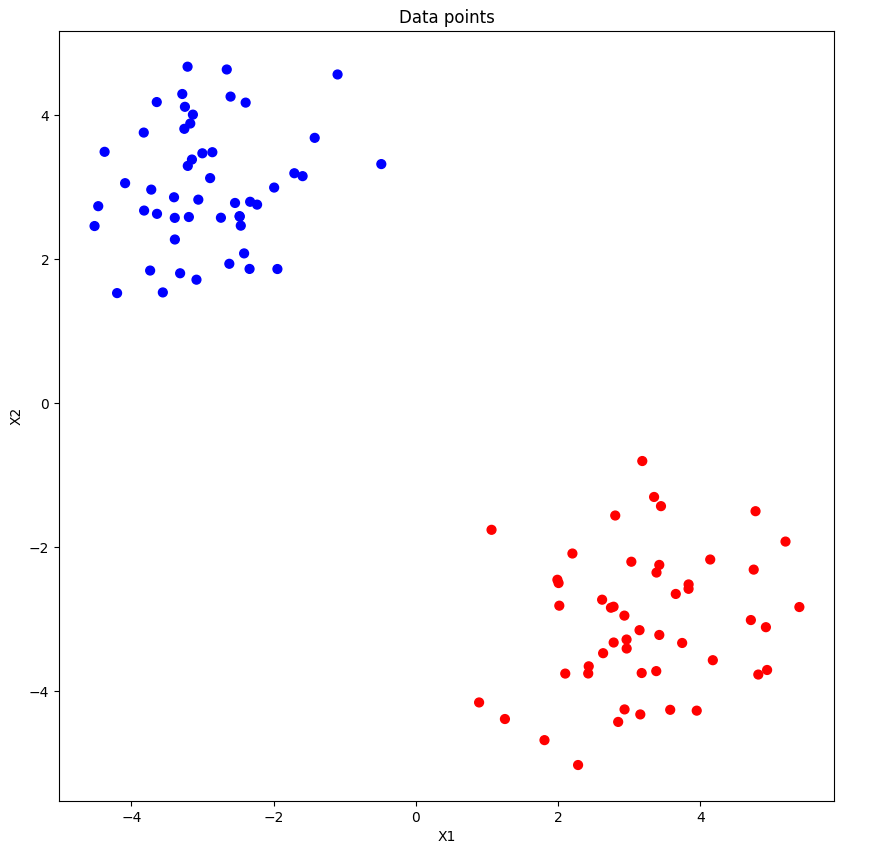
\includegraphics[width=0.9\textwidth]{figures/datapoints1.png}
	\caption{Datapoints}
	\label{datapoints1}
\end{figure}

\newpage
\begin{enumerate}[a)]
  
%%%%%%%%%%%%%%%%%%%%%%%%%% 1.1 a)
  
  \item \textbf{SVM with linear kernel}
  
\begin{figure}[H]
	\centering
  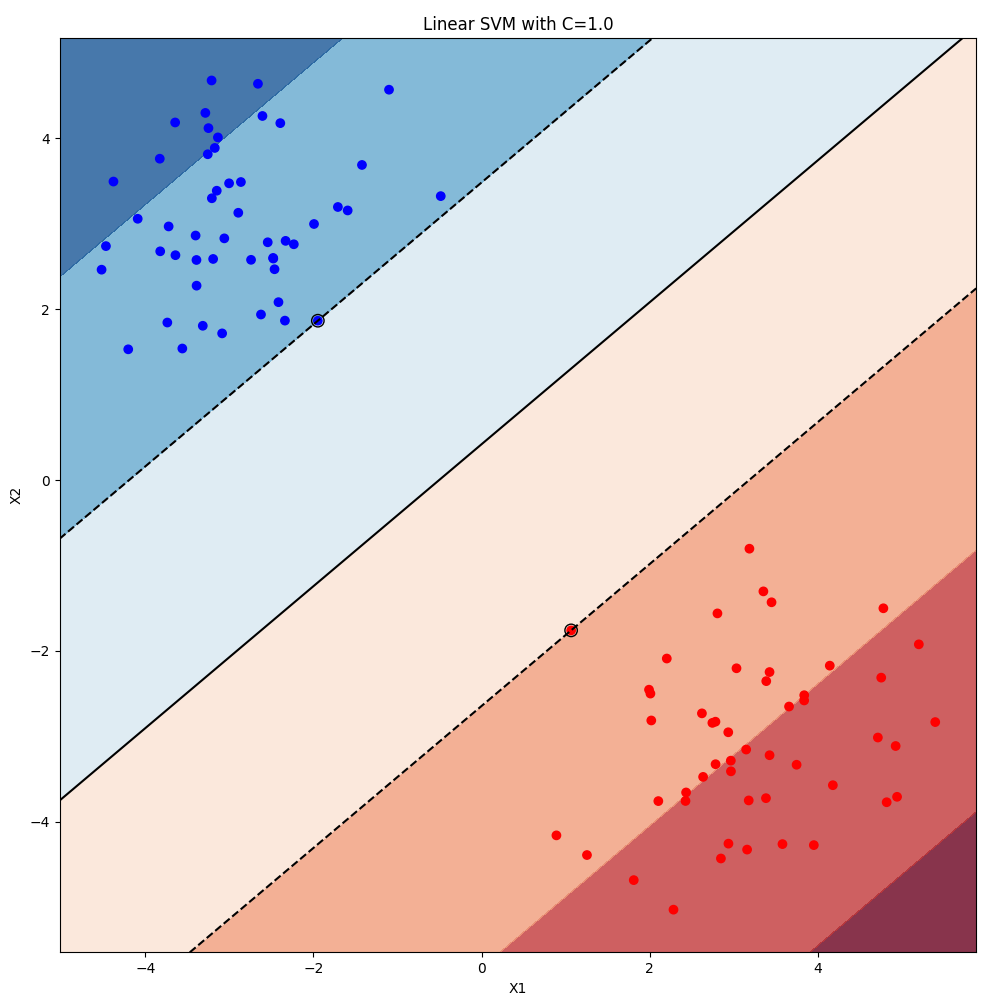
\includegraphics[width=0.9\textwidth]{figures/svm1.png}
	\caption{SVM with linear kernel}
	\label{svm1}
\end{figure}

%%%%%%%%%%%%%%%%%%%%%%%%%% 1. b)
\newpage
  \item \textbf{Regularization, balancing, noise or bad outliers}

When adding a point (e.g. $(4,0)$ for class $1$) and using parameter $C = 1$
\[default\] (panelty for error, see Figure\ \ref{svm1_b_c1} SVM will treat it
as noise since there are a lot of positive classified point compared to the negative. For
$C = 3$ see Figure\ \ref{svm1_b_c3}. Low $C$ makes a smooth decision boundary while higher $C$ aims to
maximizing correct
classification\autocite{scikit:svm}\autocite{scikit:svm_parameters}.

\begin{figure}[H]
	\centering
  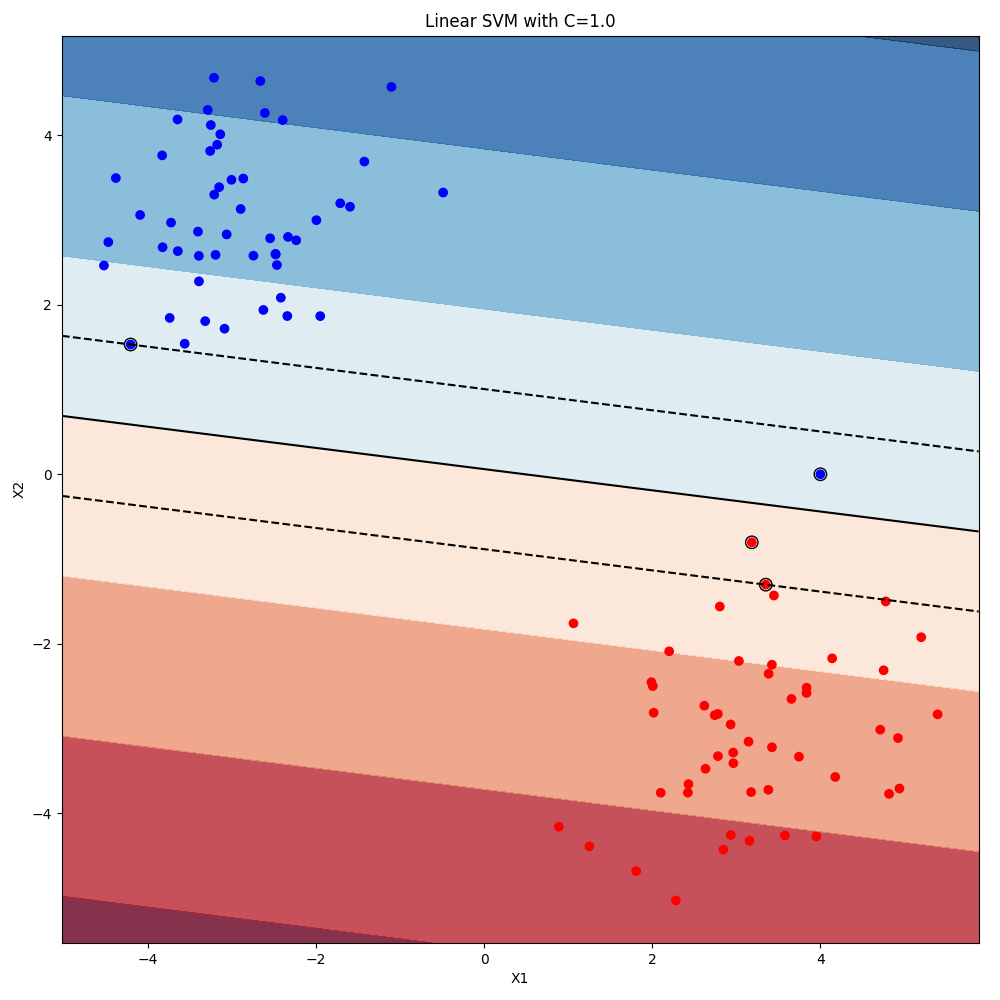
\includegraphics[width=0.5\textwidth]{figures/svm1_b_c1.png}
	\caption{SVM with linear kernel and $C=1$}
	\label{svm1_b_c1}
\end{figure}

\begin{figure}[H]
	\centering
  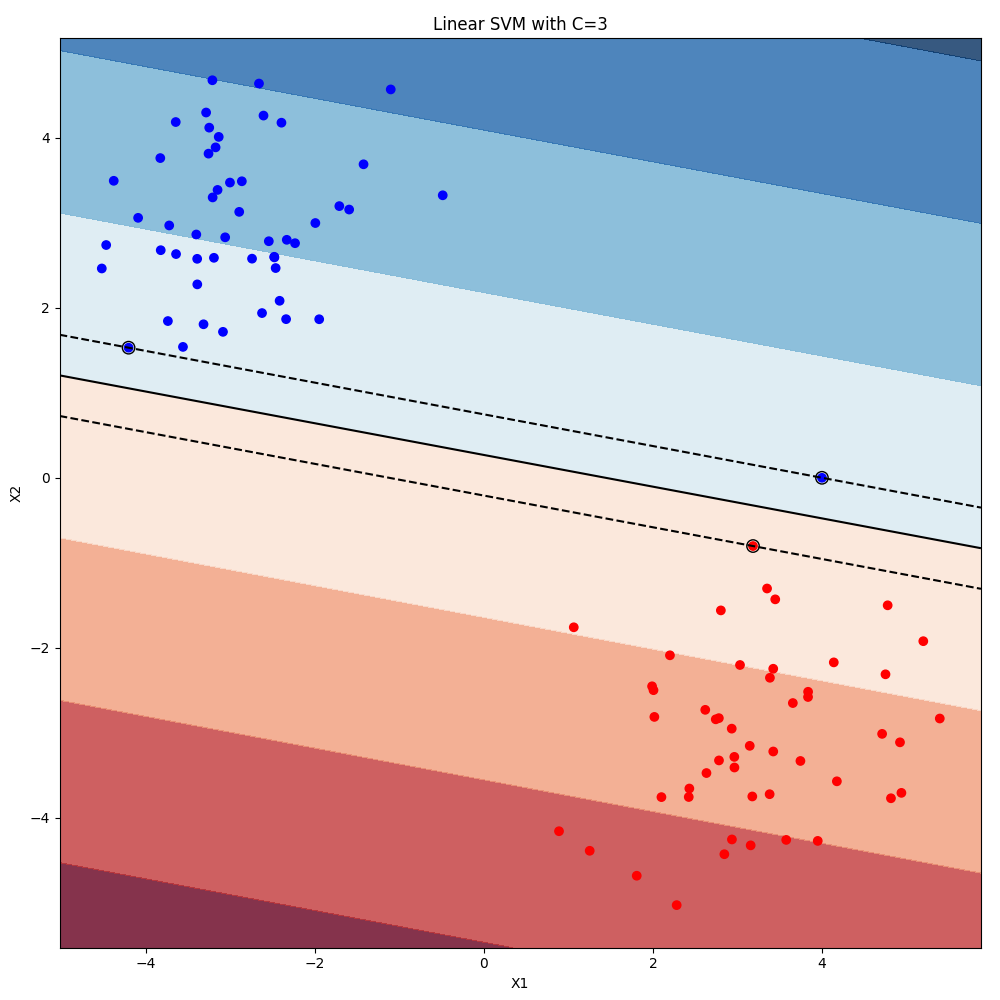
\includegraphics[width=0.5\textwidth]{figures/svm1_b_c3.png}
	\caption{SVM with linear kernel and $C=3$}
	\label{svm1_b_c3}
\end{figure}

\textbf{Discussion}

There are a number of ways to adjust parameter to suite training samples, please
see \autocite{scikit:svm_parameters} and
\autocite{scikit:svm_regularization_parameter}.

%%%%%%%%%%%%%%%%%%%%%%%%%% 1. c)
\newpage
  \item \textbf{Scaling the Regularization}

Different values for parameter $C$ can lead to either more misclassified samples
but a smooth (better) decision boundary (ecpecially in higher planes) and on the
other hand do better classification but misses sample point (since the penalty
for the error is not that high). Following are some examples for differen $C$s.

\begin{figure}[H]
	\centering
  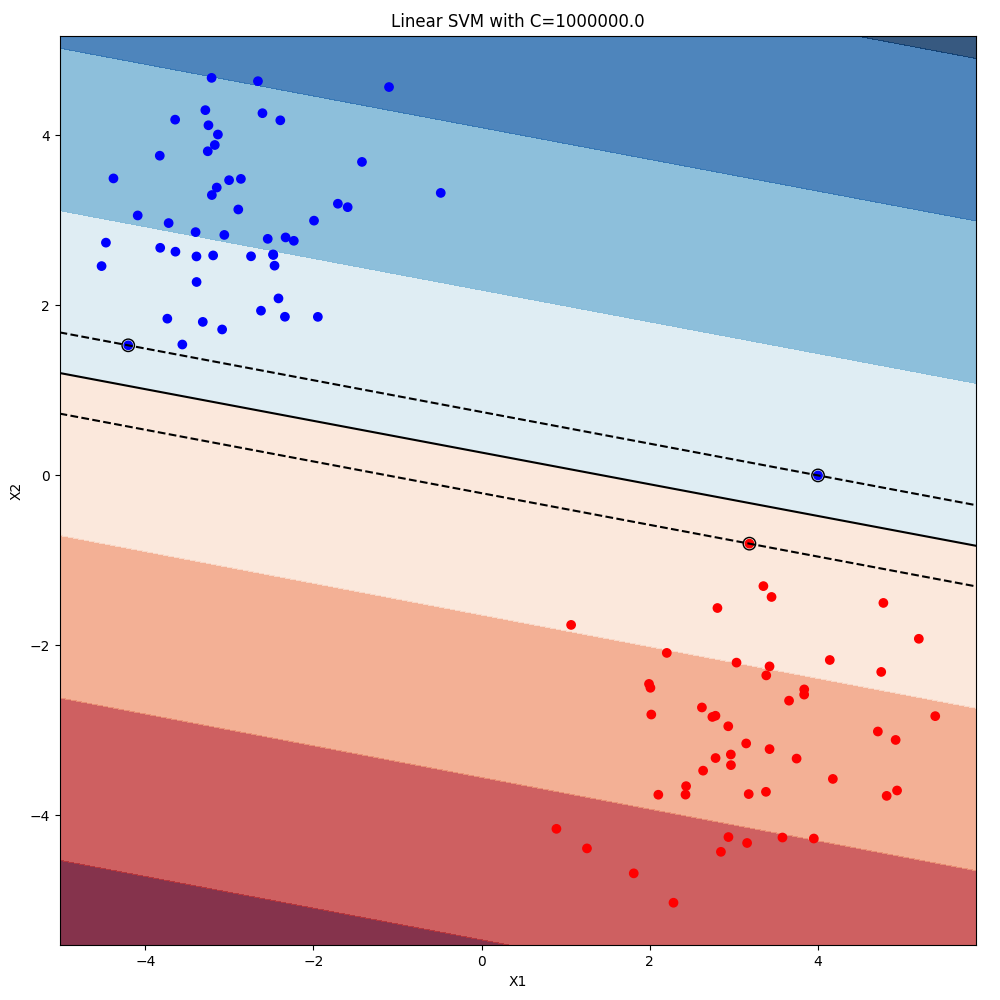
\includegraphics[width=0.6\textwidth]{figures/svm1_c_c1e6.png}
	\caption{Linear SVM $C=10^6$}
	\label{svm1_c_c1e6}
\end{figure}

\begin{figure}[H]
	\centering
  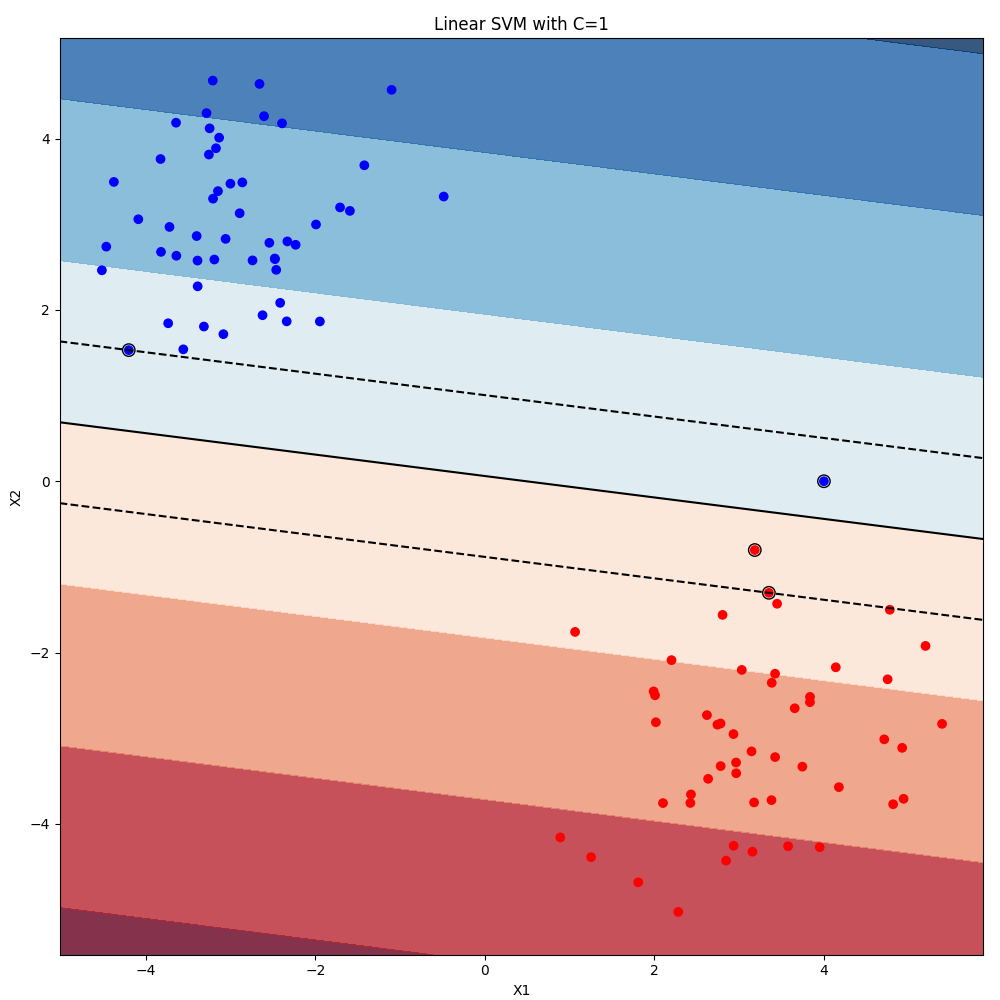
\includegraphics[width=0.6\textwidth]{figures/svm1_c_c1e0.png}
	\caption{Linear SVM $C=10^0$}
	\label{svm1_c_c1e0}
\end{figure}

\begin{figure}[H]
	\centering
  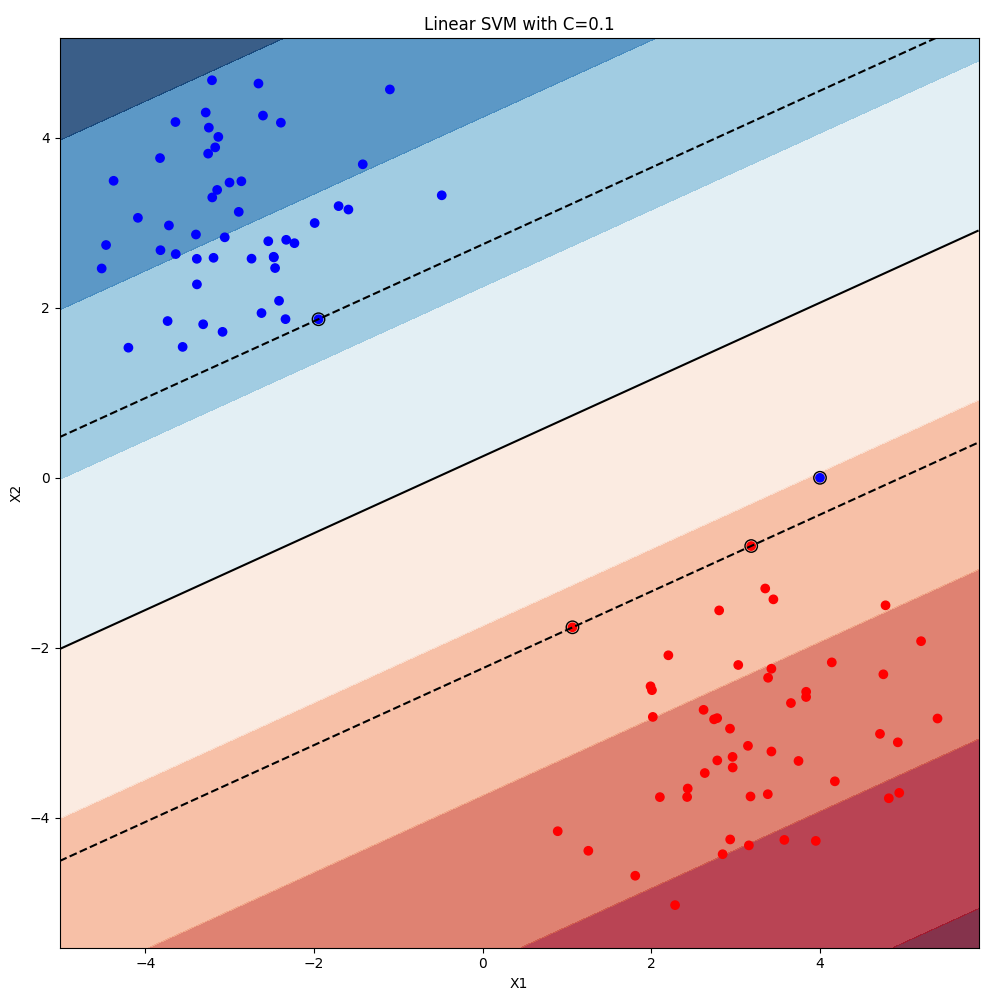
\includegraphics[width=0.6\textwidth]{figures/svm1_c_c1e-1.png}
	\caption{Linear SVM $C=10^{-1}$}
	\label{svm1_c_c1e-1}
\end{figure}

\begin{figure}[H]
	\centering
  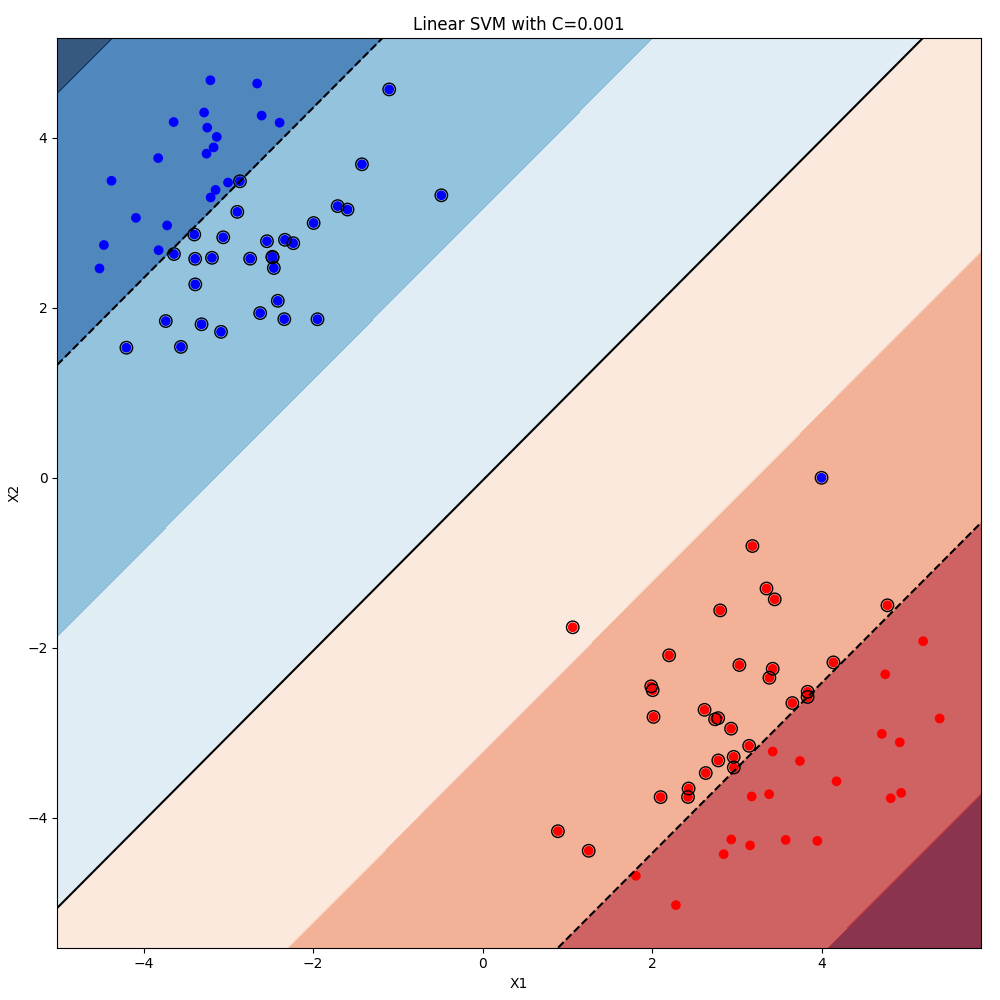
\includegraphics[width=0.6\textwidth]{figures/svm1_c_c1e-3.png}
	\caption{Linear SVM $C=10^{-3}$}
	\label{svm1_c_c1e-3}
\end{figure}

\texttt{Support Vectors (C=1000000.0): 3\\
Support Vectors (C=1): 4\\
Support Vectors (C=0.1): 4\\
Support Vectors (C=0.001): 62\\
}

\textbf{Disussion}

The number of support vectors increases with decrease of $C$ since more
missclassified sample fall within the margin. The penalty of the missclassified
samples is lower and more of them are accepted to be inside the margin.

\end{enumerate}

\newpage
\section{Non-linear (kernel) SVM}

\begin{figure}[H]
	\centering
  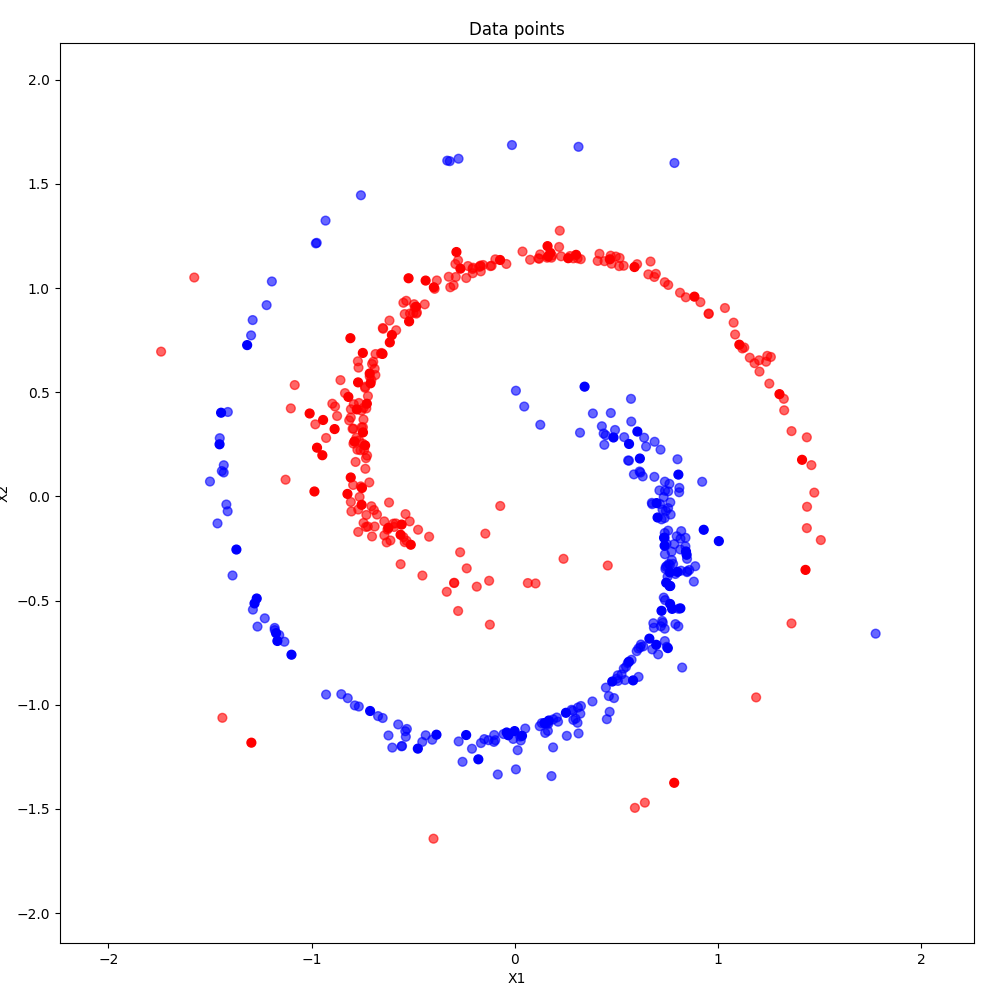
\includegraphics[width=0.9\textwidth]{figures/datapoints2.png}
	\caption{Datapoints for kernel tests}
	\label{datapoints2}
\end{figure}

\newpage
\begin{enumerate}[a)]
  
%%%%%%%%%%%%%%%%%%%%%%%%%% 2. a)
  
  \item \textbf{SVM with linear kernel}
  
\begin{figure}[H]
	\centering
  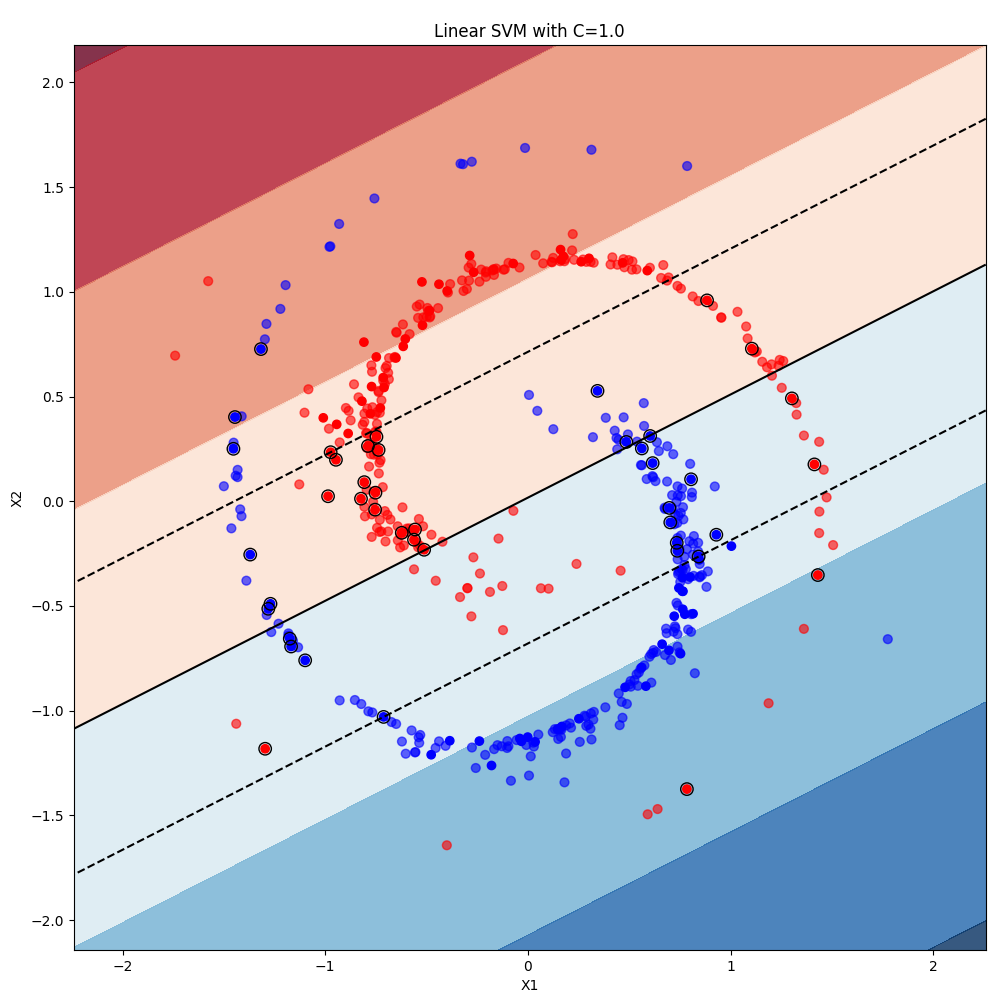
\includegraphics[width=0.9\textwidth]{figures/svm2_a_c1.png}
	\caption{Linear (kernel) SVM}
	\label{svm2_a_c1}
\end{figure}

\textbf{Result}

  Score (linear): 0.8125

\textbf{Discussion}

Fitting quite well ($0.8125$) for this weird data and usage of a linear kernel. 

%%%%%%%%%%%%%%%%%%%%%%%%%% 2. b)
\newpage
  \item \textbf{SVM with poly kernel}

SVM with polynomial kernel using different degrees and coefficient0 = 1.

\begin{figure}[H]
	\centering
  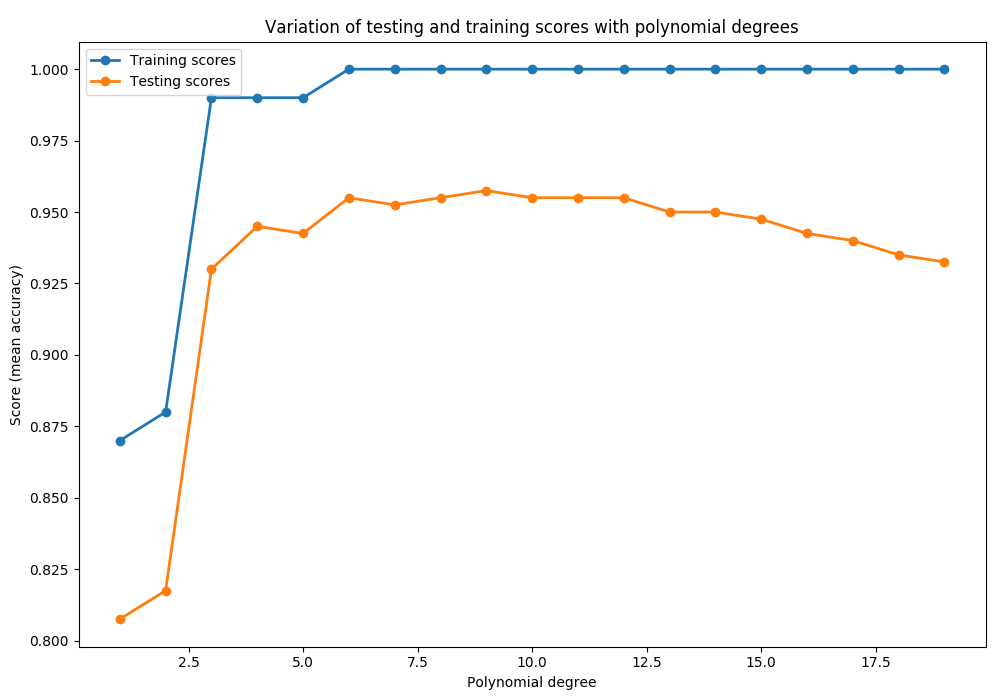
\includegraphics[width=0.9\textwidth]{figures/svm2_b_scores.png}
	\caption{Scores with different value for degree using polynomial kernel}
	\label{svm2_b_scores}
\end{figure}

\textbf{Result}

Best test score is $0.9575$ at degree $9$.

\begin{figure}[H]
	\centering
  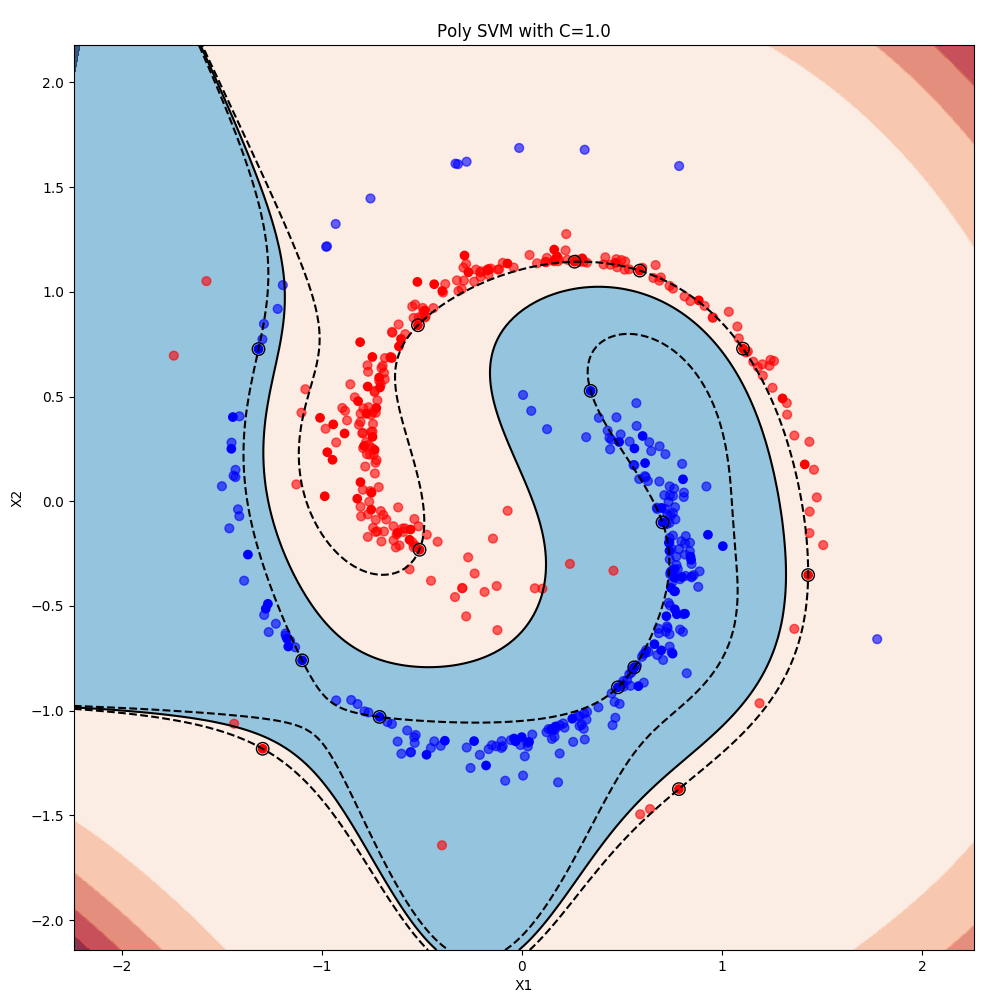
\includegraphics[width=0.9\textwidth]{figures/svm2_b_best.png}
	\caption{SVM with polynomial kernel with degree 9}
	\label{svm2_b_best}
\end{figure}

%%%%%%%%%%%%%%%%%%%%%%%%%% 2. c)
\newpage
  \item \textbf{SVM with rbf kernel}

SVM with rbf kernel using different values for $\gamma$.

\begin{figure}[H]
	\centering
  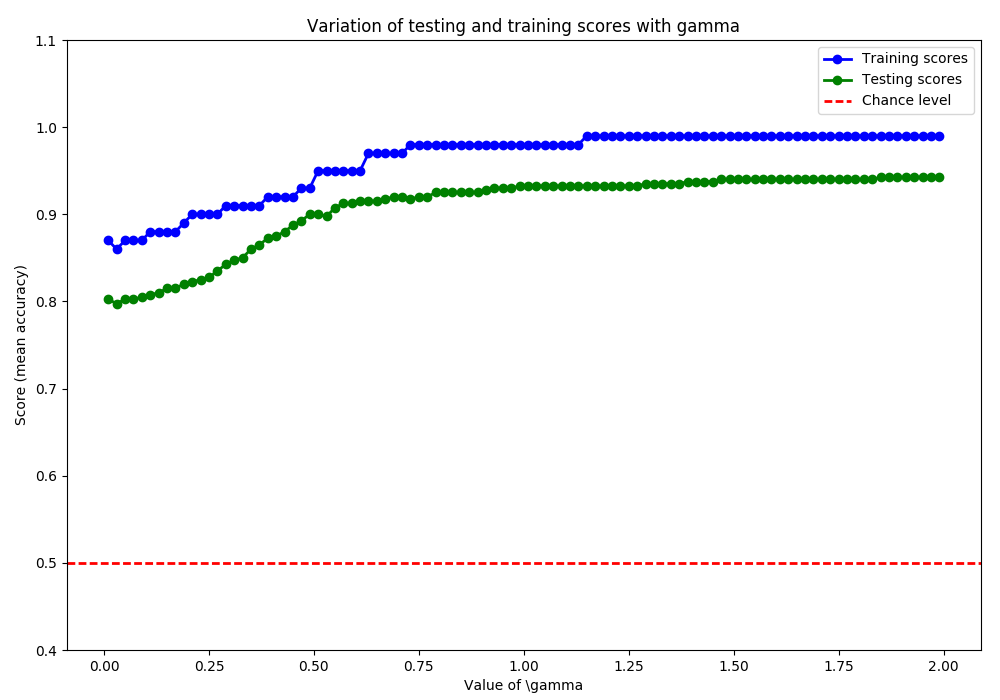
\includegraphics[width=0.9\textwidth]{figures/svm2_c_scores.png}
	\caption{Scores with different value for $\gamma$ using rbf kernel}
	\label{svm2_c_scores}
\end{figure}

\textbf{Result}

Best score is $0.9425$ at $\gamma = 1.85$

\begin{figure}[H]
	\centering
  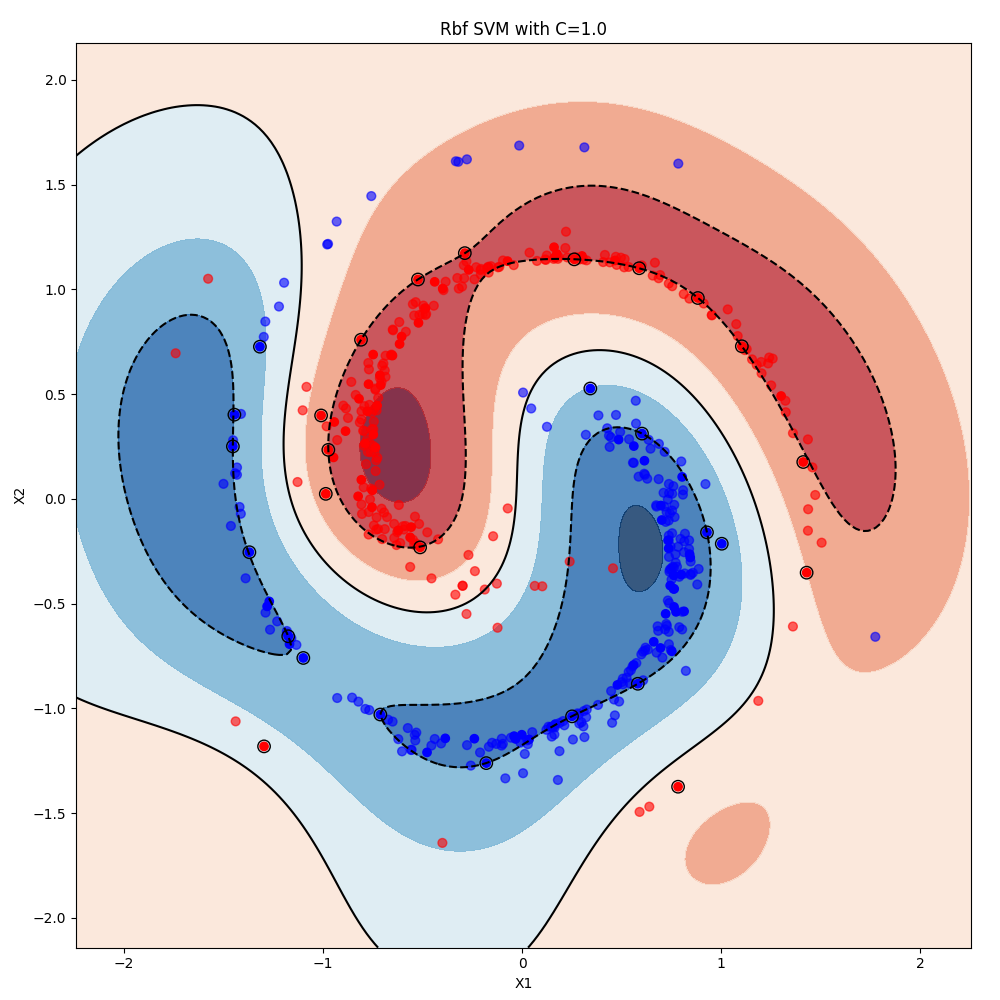
\includegraphics[width=0.9\textwidth]{figures/svm2_c_best.png}
	\caption{SVM with rbf kernel with $\gamma = 1.85$}
	\label{svm2_c_best}
\end{figure}

\textbf{Discussion}

Best score and simpliest disicion boundary can be achieved using
\textbf{polynomial} kernel at degree $9$. The maximum score with this
configuraiton is $95.75\,\%$ accuracy. Linear kernel performes best im case of
runtime but is not fitting (generalization) the data very well. Polynomial would
be the best choice for both fitting and performance. Rbf kernel is creating very
complex disicion boundaries. There are also very complex boundaries with poly
kernels at higher degrees.

\end{enumerate}

\section{Multiclass classification}

\begin{figure}[H]
	\centering
  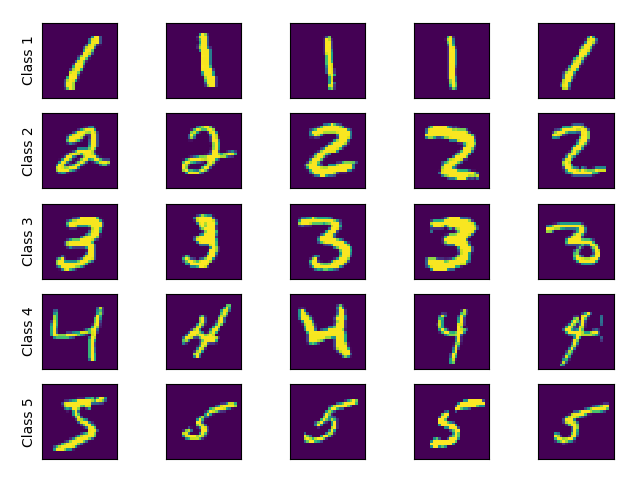
\includegraphics[width=0.9\textwidth]{figures/data3.png}
	\caption{Data for multiclass classification}
	\label{data3}
\end{figure}

\newpage
\begin{enumerate}[a)]
  
%%%%%%%%%%%%%%%%%%%%%%%%%% 3. a)
\newpage
  \item \textbf{Testing and scores (linear vs. rbf kernel)}

Using multiclass classification with scikit SVM api testing different SVMs
parametrizations. In Figure 

\begin{figure}[H]
	\centering
  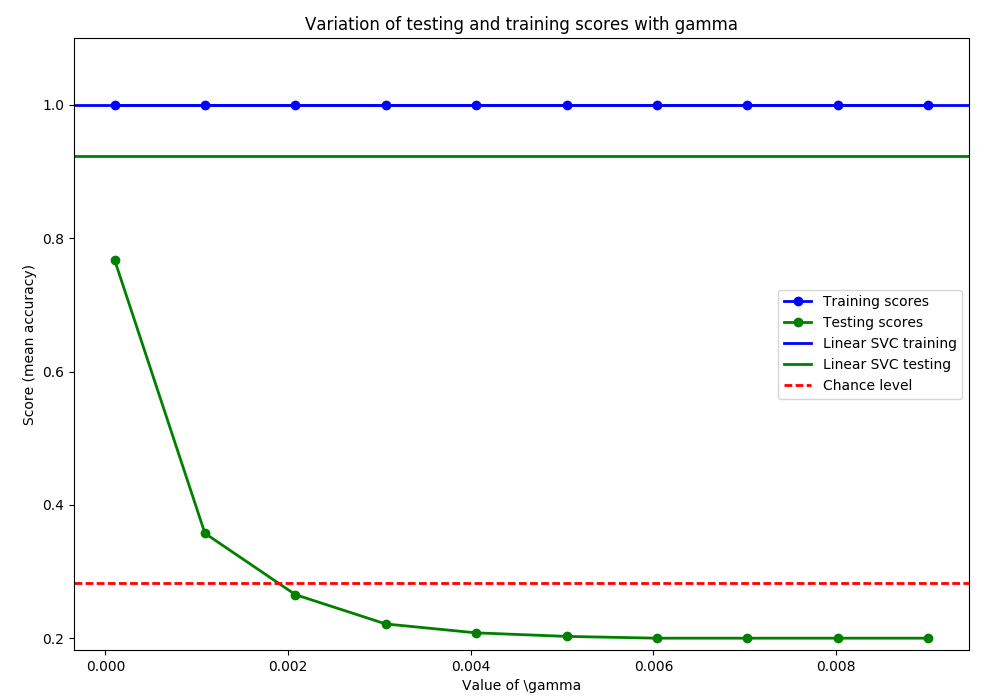
\includegraphics[width=0.9\textwidth]{figures/svm3_a_scores.png}
	\caption{Scores for SVM multiclass classification (rbf vs. linear)}
	\label{svm3_a_scores}
\end{figure}

Score (linear): $0.924$\\
Best score (rbf) is $0.768$ at $\gamma = 0.0001$

%%%%%%%%%%%%%%%%%%%%%%%%%% 3. a)
\newpage
  \item \textbf{Evaluation of missclassification}

Analyzing missclassified images:

\begin{figure}[H]
	\centering
  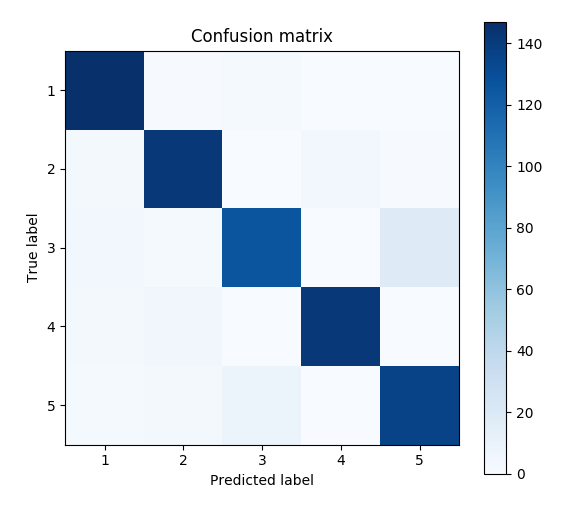
\includegraphics[width=0.6\textwidth]{figures/svm3_b_cm.png}
	\caption{Confusion matrix}
	\label{svm3_b_cm}
\end{figure}

\begin{figure}[H]
	\centering
  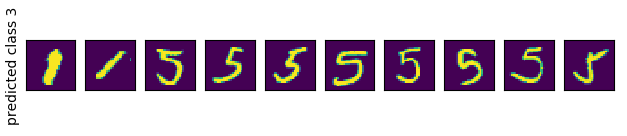
\includegraphics[width=0.8\textwidth]{figures/svm3_b_mc.png}
	\caption{Missclassified data}
	\label{svm3_b_mc}
\end{figure}

\textbf{Discussion}

\begin{itemize}
  \item[--] Recall \textbf{ovr} (one vs. all/rest) and \textbf{ovo} (one vs.
  one)
    \begin{itemize}
	  \item[\textbullet] \textbf{ovr}: Create classifiers that distinguish each
	  class from all other classes\autocite{lecuter_notes_ci}. For $\mathit{N}$ classes
	  $\mathit{N} $ classifiers must be trained.
	  \item[\textbullet] \textbf{ovo}: Create classifiers that distinguish between
	  each pair of classes\autocite{lecuter_notes_ci}. for $\mathit{N}$ classes
	  $\rightarrow \mathit{N}(\mathit{N} - 1) / 2$ classifiers must be trained.
	\end{itemize}
  \item[--] Why linear kernel: Pattern recognision in images means clustering
  and clusters for text or symbols (digits) have linear properties (curves,
  lines).
  \item[--] Highest error in $3$ vs. $5$.
  \item[--] Mistakes: Digits $3$ and $5$ have bottom curve in common. It the top
  part is not ``fine'' enouth (too narrow) there would be no second
  characteristic. Depending on the disicion boundary orientation ($k$) they
  woulb be identical in terms of SVM classification with linear kernel.
\end{itemize}

\end{enumerate}

\newpage
\printbibliography

\end{document}